\chapter{Evaluation results} \label{chap_evaluation}

This Chapter focuses on the comparison of \gls{ca} and \gls{ns} and explores the
convergence between the two architectural design approaches. We will start by comparing
the principles of \gls{ca} with the theories of \gls{ns} and analyze how they converge in
their approach and the effect on the software design. In section
\ref{sec_converging_elements}, we will compare the design elements of the two
architectural approaches. We will highlight the similarities and differences in their
implementation, in order to determine the further convergence of the two discussed
architectural design approaches.

To conduct this comparison, we used a combination of artifacts and a literature study. We
analyzed real-world examples of software artifacts that were designed using \gls{ca}, and
reviewed the relevant literature to gain a comprehensive understanding of both approaches.

Throughout this evaluation chapter, we will explore the strengths and weaknesses of each
approach, as well as the potential benefits of their convergence. By examining the
principles and design elements of \gls{ca} and \gls{ns}, we hope to provide a clear
understanding of the effects of using the different approaches in conjunction with each
other.

\section{The Convergence of Priniples} \label{sec_converging_principles}

In this section, we will apply a systematic cross-referencing approach to assess the level
of convergence between each of the principles of \gls{ca} with \gls{ns}. Along with
a brief explanation, the level of convergence is denoted as follows:

\begin{table}[H]
    \begin{tabular}{ l l p{0.57\linewidth}} Fully converges & \conv & This indicates that
    the principles of \gls{ca} and \gls{ns} are highly aligned. Both have a similar impact
    on the design and implementation of the artifact. \\
        
        Supports convergence & \partconv & The \gls{ca} principle supports in implementing
        the \gls{ns} principle through specific design choices. However, applying the
        \gls{ca} principle does not inherently ensure adherence to the corresponding
        \gls{ns} principle. \\
        
        No convergence & \noconv & There appears to be a discrepancy between the \gls{ca}
        principle and its corresponding \gls{ns} principle. \\
    \end{tabular}
\end{table}

\subsection{Single Responsibility Principle} \label{srp}

\evaluatePrincipleTable{\gls{srp}}{table_srp_alignment}{ \addEvalRow{\gls{soc} & \fullAlignment &
    The main goal of both \gls{srp} and \gls{soc} is to promote and encourage modularity,
    low coupling, and high cohesion. While the definition has some differences, the two
    principles can be regarded as practically interchangeable. Many examples in the
    Artifacts show a strong alignment between \gls{srp} and \gls{soc}. To name one, an
    Expander should be able to can perform multiple Tasks to complete the full
    instantiation of the Model. Each of those Tasks can be implemented separately from
    each other. Figure \ref{fig_handlers} illustrated some of the Tasks that are
    implemented in the Clean Architecture Expander Artifact. The Code Listing
    \ref{list_entityexpander} is an example of one implementation of such a Task
    \citecode{koks_expandentitieshandlerinteractor_2023}.}
    
    \addEvalRow{\gls{dvt} & \partialAlignment & Although using \gls{srp} does not
    implicitly guarantees \gls{dvt}, it does support \gls{dvt} by directing certain design
    choices. For example, both \gls{ca} and \gls{ns} assign specific \gls{dto} objects to
    support specific use cases (Interactors or Tasks) or to transfer (parts of) Data
    between architectural layers. \gls{ca} specifically assigned \glspl{dto} and
    guidelines on where and when to use them. These are also applied in the Artifact of
    this study as ResponseModels, RequestModels, and ViewModels
    \parencites{koks_requestmodels_2023,koks_viewmodels_2023}. The separation of data
    structures specific to Use Cases minimizes the impact of data structure changes by
    preferring stamp coupling over data coupling. However, \gls{srp} is not a guaranteed
    measure for \gls{dvt}.}
    
    \addEvalRow{\gls{avt} & \partialAlignment & While \gls{srp} emphasizes limiting the
    responsibility of each module, it does not explicitly require handling specific
    versions of use cases. Nevertheless, adhering to gls{srp} can still indirectly
    contribute to achieving \gls{avt}. One way to achieve this is by separating versions
    of Actions into separate contracts, objects, or methods, enabling Action Version
    transparency to some degree. Although not yet available in the Artifact, the Code
    Listing \ref{list_versioning} shows that API versioning is a common standard practice
    and fully supported by the open API specifcation and the .net core framework
    \parencites{github_aspnet-api-versioningprogramcs_2023, oas_versioning_2023}.
    Manifestations in the Artifact can be located in the Logger (Code Listing
    \ref{list_logging}), amongst others \parencite*{koks_logger_2023}.}
    
    \addEvalRow{\gls{sos} &\noAlignment & Following \gls{srp} might lead to separate modules
    that manage their state, indirectly contributing to \gls{sos}. However, the alignment
    is very weak, and no manifestations are found in the artifacts.}

}

\begin{figure}[H]
    \centering
    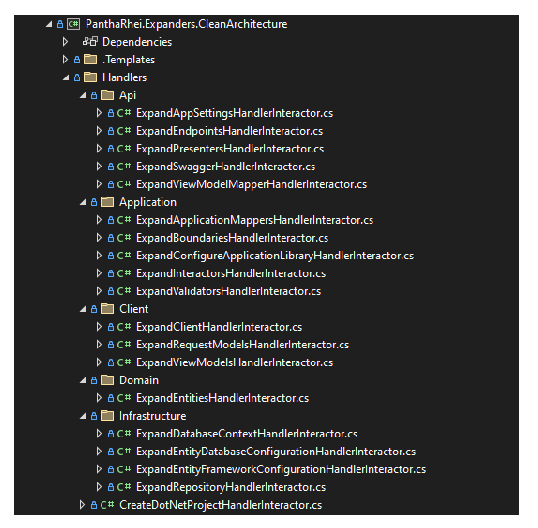
\includegraphics[width=0.6\textwidth]{figures/expander_handlers.pdf}
    \caption[handlers]{Each of the handlers handles an isolated part of the expanding process.}
    \label{fig_handlers}
\end{figure}
\subsection{Open/Closed Principle}

\evaluatePrincipleTable{\acrshort{ocp}}{table_ocp_convergence}{ 
    
\addEvalRow{\gls{soc} & \fullConvergence & The \gls{ocp} strongly converges with
    the \gls{soc} principle of \gls{ns}. \gls{ocp} states that software architectures
    should be open for extension but closed for modification. When applying \gls{ocp}
    correctly, the architecture supports new requirements built as an extension, affecting
    as few existing implementations as possible. Conversely, adhering to \gls{soc} does
    not guarantee adherence to \gls{ocp}, as \gls{soc} focuses on modularization and
    encapsulation rather than the extensibility of functionality. The same example with
    the Tasks provided in sub-section \ref{srp} is also an excellent manifestation of this
    principle.} 
    
\addEvalRow{\gls{dvt} & \noConvergence & The \gls{ocp} indirectly relates to the \gls{dvt}
principle. The convergence of both principles is weak, and no manifestations are found in
the artifacts.}
    
\addEvalRow{\gls{avt} & \fullConvergence & The \gls{ocp} strongly converges with the
    \gls{avt} principle of \gls{ns}, as both principles emphasize the importance of
    allowing changes or extensions to actions without affecting existing implementations.
    \gls{ocp} is also closely related to \gls{srp}. Besides \gls{srp}, \gls{ocp} has the
    most manifestations in the artifact, some of which are already mentioned in previous
    examples. } 
    
\addEvalRow{\gls{sos} & \noConvergence & The \gls{ocp} indirectly relates to the \gls{sos}
    principle. The convergence of both principles is weak, and no manifestations are found
    in the artifacts. } }
\subsection{Liskov Substitution Principle}

\evaluatePrincipleTable{\gls{lsp}}{table_lsp_alignment}{ 
    
\addEvalRow{\gls{soc} & \fullAlignment & \gls{lsp} states that objects of a derived class should be
able to replace objects of the base class without affecting the program negatively.
Replacing objects can only be achieved by separating them, aligning the principles
inherritly. A good example is the implementation of the
\citecode{koks_itemplateinteractor_2023} where the template engine Scriban
\parencite{github_scriban_2023} is used to generate code instantiations as a result of the
Expanding the Model \parencite{koks_scribantemplateinteractor_2023}. We could easily
replace the Scriban template engine for an other engine with only impacting the Dependency
Injection Register.}
    
\addEvalRow{\gls{dvt} & \noAlignment & The alignment between \gls{lsp} and \gls{dvt} is weak,
and no manifestations are found in the artifacts.}
    
\addEvalRow{\gls{avt} & \partialAlignment & The \gls{lsp} supports the \gls{avt} principle.
Both principles emphasize the importance of allowing the extensibility of the software
system. By adhering to \gls{lsp}, the architecture allows for class hierarchies that can
be easily extended to accommodate new (versions of) actions, which can contribute to
achieving \gls{avt}. However, adhering to \gls{lsp} alone may not guarantee full adherence
with \gls{avt}. Considder \citecode{koks_icreategateway_2023} in Code Listing
\ref{list_ICreateGatewayExamples}. The artifact contains multiple implementations of this
interface. Each implementation could be considered a different version applied to the
interface.} 
    
\addEvalRow{\gls{sos} & \noAlignment & The \gls{lsp} does not relate to the \gls{sos}
principle. The alignment of both principles is weak, and no manifestations are found in
the artifacts.} }

\subsection{Interface Segregation Principle}

\evaluatePrincipleTable{\gls{isp}}{table_isp_convergence}{ 
    
\addEvalRow{\gls{soc} & \fullConvergence & The \gls{isp} strongly converges with the
\gls{soc} principle, as both emphasize the importance of modularity and the separation of
concerns. \gls{isp} states that clients should not be forced to depend on implementation
they do not use, promoting the creation of smaller, focused interfaces. Listing
\ref{list_ispexample} shows that each \gls{crud} operation has its own interface
\parencite{koks_crudgateways_2023}.}
    
\addEvalRow{\gls{dvt} & \noConvergence & The \gls{isp} does not relate to the \gls{dvt}
principle. The convergence of both principles is weak, and no manifestations are found in
the artifacts.}
    
\addEvalRow{\gls{avt} & \npartialConvergence & The convergence between \gls{isp} and
\gls{avt} arises from the emphasis of \gls{isp} on creating targeted interfaces tailored
to specific needs. Smaller interfaces can enhance modularity and minimize unwanted side
effects when modifying Actions in the software system, positively impacting the
implementation of the \gls{avt}. For example, modifications in Actions are likely to have
a limited impact. However, adhering to \gls{isp} is not a guarantee for \gls{avt}.} 
    
\addEvalRow{\gls{sos} & \noConvergence & The \gls{isp} does not relate to the \gls{sos}
principle. The convergence of both principles is weak, and no manifestations are found in
the artifacts.} 

}
\subsubsection{The Dependency Inversion Principle} \label{subsubsec_dip} 
\textcolor{red}{
TODO: explain how dependency injection can benefit the implementation and align with
\ref{tab_convergence_dip}}

The \gls{dip} prescribes that high-level modules should not depend on low-level modules,
and that both should depend on abstractions. The principle emphasizes that the
architecture should be designed in such a way that the flow of control between the
different objects, layers and components are always from higher-level implementations
to lower-level details.

In other words, high-level implementations like business rules, should not be concerned
about low-level implementations, such as the way the data is stored or presented to the
end user. Additionally, both the high-level and low-level implementations should only
depend on abstractions or interfaces that define a contract for how they should interact
with each other \parencite[109]{robert_c_martin_clean_2018}.

This approach allows for great flexibility and a modular architecture. Modifications in
the low-level implementations will not affect the high-level implementations as long as
they still adhere to the contract defined by the abstractions and interfaces.
Similarly, changes to the high-level modules will not affect the low-level modules as long
as they still fulfill the contract. This reduces coupling and ensures the evolvability
system over time, as changes can be made to specific modules without affecting the rest of
the system.

Manifestations in the artifacts are ample. One of which is the consistent use of the
Dependency Injection pattern. In order to prevent the risks of displacing and dispersing
dependencies all over the system \parencite[214]{mannaert_normalized_2016} we are using
dependency containers. Each module is maintaining its own dependencies, which are
bootstrapped at application startup (see Listing \ref{list_dip})
\parencite{koks_generator_2023}.

\lstinputlisting[
    caption={Bootstrapping the dependencies of each component/layer of the
    generator artifact.},
    label={list_dip}]
    {Snippets/Dip.cs}

A more abstract example is the separation of required modules into separate component
libraries. This applies to both the generated and generator artifact (see Figure
\ref{fig_solutions}). The actual compliance to the \gls{dip} is how the flow of control
between the components is organized. This is accurately depicted in Figure
\ref{fig_modulair_components} \nameref{fig_modulair_components}.

\begin{figure}[H]
    \centering
    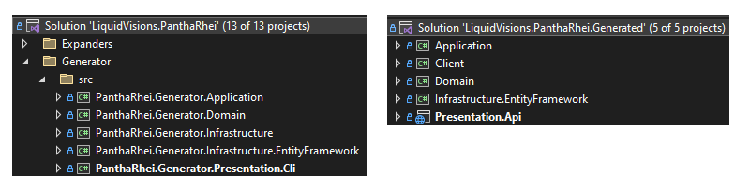
\includegraphics[width=1\textwidth]{figures/solutions.pdf}
    \caption[Separation of component libraries]{Separation of component libraries.}
    \label{fig_solutions}
\end{figure}
\subsection{Single Responsibility Principle} \label{srp}

\evaluatePrincipleTable{\gls{srp}}{table_srp_alignment}{ \addEvalRow{\gls{soc} & \fullAlignment &
    The main goal of both \gls{srp} and \gls{soc} is to promote and encourage modularity,
    low coupling, and high cohesion. While the definition has some differences, the two
    principles can be regarded as practically interchangeable. Many examples in the
    Artifacts show a strong alignment between \gls{srp} and \gls{soc}. To name one, an
    Expander should be able to can perform multiple Tasks to complete the full
    instantiation of the Model. Each of those Tasks can be implemented separately from
    each other. Figure \ref{fig_handlers} illustrated some of the Tasks that are
    implemented in the Clean Architecture Expander Artifact. The Code Listing
    \ref{list_entityexpander} is an example of one implementation of such a Task
    \citecode{koks_expandentitieshandlerinteractor_2023}.}
    
    \addEvalRow{\gls{dvt} & \partialAlignment & Although using \gls{srp} does not
    implicitly guarantees \gls{dvt}, it does support \gls{dvt} by directing certain design
    choices. For example, both \gls{ca} and \gls{ns} assign specific \gls{dto} objects to
    support specific use cases (Interactors or Tasks) or to transfer (parts of) Data
    between architectural layers. \gls{ca} specifically assigned \glspl{dto} and
    guidelines on where and when to use them. These are also applied in the Artifact of
    this study as ResponseModels, RequestModels, and ViewModels
    \parencites{koks_requestmodels_2023,koks_viewmodels_2023}. The separation of data
    structures specific to Use Cases minimizes the impact of data structure changes by
    preferring stamp coupling over data coupling. However, \gls{srp} is not a guaranteed
    measure for \gls{dvt}.}
    
    \addEvalRow{\gls{avt} & \partialAlignment & While \gls{srp} emphasizes limiting the
    responsibility of each module, it does not explicitly require handling specific
    versions of use cases. Nevertheless, adhering to gls{srp} can still indirectly
    contribute to achieving \gls{avt}. One way to achieve this is by separating versions
    of Actions into separate contracts, objects, or methods, enabling Action Version
    transparency to some degree. Although not yet available in the Artifact, the Code
    Listing \ref{list_versioning} shows that API versioning is a common standard practice
    and fully supported by the open API specifcation and the .net core framework
    \parencites{github_aspnet-api-versioningprogramcs_2023, oas_versioning_2023}.
    Manifestations in the Artifact can be located in the Logger (Code Listing
    \ref{list_logging}), amongst others \parencite*{koks_logger_2023}.}
    
    \addEvalRow{\gls{sos} &\noAlignment & Following \gls{srp} might lead to separate modules
    that manage their state, indirectly contributing to \gls{sos}. However, the alignment
    is very weak, and no manifestations are found in the artifacts.}

}

\begin{figure}[H]
    \centering
    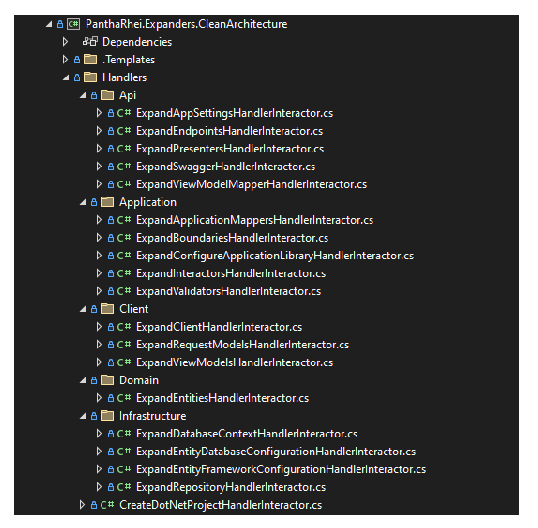
\includegraphics[width=0.6\textwidth]{figures/expander_handlers.pdf}
    \caption[handlers]{Each of the handlers handles an isolated part of the expanding process.}
    \label{fig_handlers}
\end{figure}
\subsection{Open/Closed Principle}

\evaluatePrincipleTable{\acrshort{ocp}}{table_ocp_convergence}{ 
    
\addEvalRow{\gls{soc} & \fullConvergence & The \gls{ocp} strongly converges with
    the \gls{soc} principle of \gls{ns}. \gls{ocp} states that software architectures
    should be open for extension but closed for modification. When applying \gls{ocp}
    correctly, the architecture supports new requirements built as an extension, affecting
    as few existing implementations as possible. Conversely, adhering to \gls{soc} does
    not guarantee adherence to \gls{ocp}, as \gls{soc} focuses on modularization and
    encapsulation rather than the extensibility of functionality. The same example with
    the Tasks provided in sub-section \ref{srp} is also an excellent manifestation of this
    principle.} 
    
\addEvalRow{\gls{dvt} & \noConvergence & The \gls{ocp} indirectly relates to the \gls{dvt}
principle. The convergence of both principles is weak, and no manifestations are found in
the artifacts.}
    
\addEvalRow{\gls{avt} & \fullConvergence & The \gls{ocp} strongly converges with the
    \gls{avt} principle of \gls{ns}, as both principles emphasize the importance of
    allowing changes or extensions to actions without affecting existing implementations.
    \gls{ocp} is also closely related to \gls{srp}. Besides \gls{srp}, \gls{ocp} has the
    most manifestations in the artifact, some of which are already mentioned in previous
    examples. } 
    
\addEvalRow{\gls{sos} & \noConvergence & The \gls{ocp} indirectly relates to the \gls{sos}
    principle. The convergence of both principles is weak, and no manifestations are found
    in the artifacts. } }
\subsection{Liskov Substitution Principle}

\evaluatePrincipleTable{\gls{lsp}}{table_lsp_alignment}{ 
    
\addEvalRow{\gls{soc} & \fullAlignment & \gls{lsp} states that objects of a derived class should be
able to replace objects of the base class without affecting the program negatively.
Replacing objects can only be achieved by separating them, aligning the principles
inherritly. A good example is the implementation of the
\citecode{koks_itemplateinteractor_2023} where the template engine Scriban
\parencite{github_scriban_2023} is used to generate code instantiations as a result of the
Expanding the Model \parencite{koks_scribantemplateinteractor_2023}. We could easily
replace the Scriban template engine for an other engine with only impacting the Dependency
Injection Register.}
    
\addEvalRow{\gls{dvt} & \noAlignment & The alignment between \gls{lsp} and \gls{dvt} is weak,
and no manifestations are found in the artifacts.}
    
\addEvalRow{\gls{avt} & \partialAlignment & The \gls{lsp} supports the \gls{avt} principle.
Both principles emphasize the importance of allowing the extensibility of the software
system. By adhering to \gls{lsp}, the architecture allows for class hierarchies that can
be easily extended to accommodate new (versions of) actions, which can contribute to
achieving \gls{avt}. However, adhering to \gls{lsp} alone may not guarantee full adherence
with \gls{avt}. Considder \citecode{koks_icreategateway_2023} in Code Listing
\ref{list_ICreateGatewayExamples}. The artifact contains multiple implementations of this
interface. Each implementation could be considered a different version applied to the
interface.} 
    
\addEvalRow{\gls{sos} & \noAlignment & The \gls{lsp} does not relate to the \gls{sos}
principle. The alignment of both principles is weak, and no manifestations are found in
the artifacts.} }

\subsection{Interface Segregation Principle}

\evaluatePrincipleTable{\gls{isp}}{table_isp_convergence}{ 
    
\addEvalRow{\gls{soc} & \fullConvergence & The \gls{isp} strongly converges with the
\gls{soc} principle, as both emphasize the importance of modularity and the separation of
concerns. \gls{isp} states that clients should not be forced to depend on implementation
they do not use, promoting the creation of smaller, focused interfaces. Listing
\ref{list_ispexample} shows that each \gls{crud} operation has its own interface
\parencite{koks_crudgateways_2023}.}
    
\addEvalRow{\gls{dvt} & \noConvergence & The \gls{isp} does not relate to the \gls{dvt}
principle. The convergence of both principles is weak, and no manifestations are found in
the artifacts.}
    
\addEvalRow{\gls{avt} & \npartialConvergence & The convergence between \gls{isp} and
\gls{avt} arises from the emphasis of \gls{isp} on creating targeted interfaces tailored
to specific needs. Smaller interfaces can enhance modularity and minimize unwanted side
effects when modifying Actions in the software system, positively impacting the
implementation of the \gls{avt}. For example, modifications in Actions are likely to have
a limited impact. However, adhering to \gls{isp} is not a guarantee for \gls{avt}.} 
    
\addEvalRow{\gls{sos} & \noConvergence & The \gls{isp} does not relate to the \gls{sos}
principle. The convergence of both principles is weak, and no manifestations are found in
the artifacts.} 

}
\subsubsection{The Dependency Inversion Principle} \label{subsubsec_dip} 
\textcolor{red}{
TODO: explain how dependency injection can benefit the implementation and align with
\ref{tab_convergence_dip}}

The \gls{dip} prescribes that high-level modules should not depend on low-level modules,
and that both should depend on abstractions. The principle emphasizes that the
architecture should be designed in such a way that the flow of control between the
different objects, layers and components are always from higher-level implementations
to lower-level details.

In other words, high-level implementations like business rules, should not be concerned
about low-level implementations, such as the way the data is stored or presented to the
end user. Additionally, both the high-level and low-level implementations should only
depend on abstractions or interfaces that define a contract for how they should interact
with each other \parencite[109]{robert_c_martin_clean_2018}.

This approach allows for great flexibility and a modular architecture. Modifications in
the low-level implementations will not affect the high-level implementations as long as
they still adhere to the contract defined by the abstractions and interfaces.
Similarly, changes to the high-level modules will not affect the low-level modules as long
as they still fulfill the contract. This reduces coupling and ensures the evolvability
system over time, as changes can be made to specific modules without affecting the rest of
the system.

Manifestations in the artifacts are ample. One of which is the consistent use of the
Dependency Injection pattern. In order to prevent the risks of displacing and dispersing
dependencies all over the system \parencite[214]{mannaert_normalized_2016} we are using
dependency containers. Each module is maintaining its own dependencies, which are
bootstrapped at application startup (see Listing \ref{list_dip})
\parencite{koks_generator_2023}.

\lstinputlisting[
    caption={Bootstrapping the dependencies of each component/layer of the
    generator artifact.},
    label={list_dip}]
    {Snippets/Dip.cs}

A more abstract example is the separation of required modules into separate component
libraries. This applies to both the generated and generator artifact (see Figure
\ref{fig_solutions}). The actual compliance to the \gls{dip} is how the flow of control
between the components is organized. This is accurately depicted in Figure
\ref{fig_modulair_components} \nameref{fig_modulair_components}.

\begin{figure}[H]
    \centering
    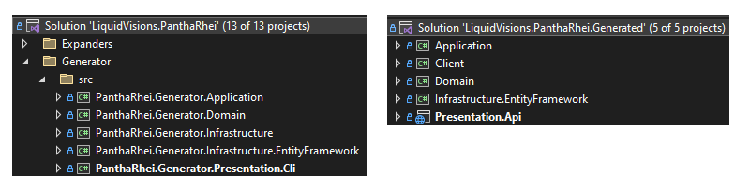
\includegraphics[width=1\textwidth]{figures/solutions.pdf}
    \caption[Separation of component libraries]{Separation of component libraries.}
    \label{fig_solutions}
\end{figure}


\section{The Convergence of Priniples} \label{sec_converging_principles}

In this section, we will apply a systematic cross-referencing approach to assess the level
of convergence between each of the principles of \gls{ca} with \gls{ns}. Along with
a brief explanation, the level of convergence is denoted as follows:

\begin{table}[H]
    \begin{tabular}{ l l p{0.57\linewidth}} Fully converges & \conv & This indicates that
    the principles of \gls{ca} and \gls{ns} are highly aligned. Both have a similar impact
    on the design and implementation of the artifact. \\
        
        Supports convergence & \partconv & The \gls{ca} principle supports in implementing
        the \gls{ns} principle through specific design choices. However, applying the
        \gls{ca} principle does not inherently ensure adherence to the corresponding
        \gls{ns} principle. \\
        
        No convergence & \noconv & There appears to be a discrepancy between the \gls{ca}
        principle and its corresponding \gls{ns} principle. \\
    \end{tabular}
\end{table}

\subsection{Single Responsibility Principle} \label{srp}

\evaluatePrincipleTable{\gls{srp}}{table_srp_alignment}{ \addEvalRow{\gls{soc} & \fullAlignment &
    The main goal of both \gls{srp} and \gls{soc} is to promote and encourage modularity,
    low coupling, and high cohesion. While the definition has some differences, the two
    principles can be regarded as practically interchangeable. Many examples in the
    Artifacts show a strong alignment between \gls{srp} and \gls{soc}. To name one, an
    Expander should be able to can perform multiple Tasks to complete the full
    instantiation of the Model. Each of those Tasks can be implemented separately from
    each other. Figure \ref{fig_handlers} illustrated some of the Tasks that are
    implemented in the Clean Architecture Expander Artifact. The Code Listing
    \ref{list_entityexpander} is an example of one implementation of such a Task
    \citecode{koks_expandentitieshandlerinteractor_2023}.}
    
    \addEvalRow{\gls{dvt} & \partialAlignment & Although using \gls{srp} does not
    implicitly guarantees \gls{dvt}, it does support \gls{dvt} by directing certain design
    choices. For example, both \gls{ca} and \gls{ns} assign specific \gls{dto} objects to
    support specific use cases (Interactors or Tasks) or to transfer (parts of) Data
    between architectural layers. \gls{ca} specifically assigned \glspl{dto} and
    guidelines on where and when to use them. These are also applied in the Artifact of
    this study as ResponseModels, RequestModels, and ViewModels
    \parencites{koks_requestmodels_2023,koks_viewmodels_2023}. The separation of data
    structures specific to Use Cases minimizes the impact of data structure changes by
    preferring stamp coupling over data coupling. However, \gls{srp} is not a guaranteed
    measure for \gls{dvt}.}
    
    \addEvalRow{\gls{avt} & \partialAlignment & While \gls{srp} emphasizes limiting the
    responsibility of each module, it does not explicitly require handling specific
    versions of use cases. Nevertheless, adhering to gls{srp} can still indirectly
    contribute to achieving \gls{avt}. One way to achieve this is by separating versions
    of Actions into separate contracts, objects, or methods, enabling Action Version
    transparency to some degree. Although not yet available in the Artifact, the Code
    Listing \ref{list_versioning} shows that API versioning is a common standard practice
    and fully supported by the open API specifcation and the .net core framework
    \parencites{github_aspnet-api-versioningprogramcs_2023, oas_versioning_2023}.
    Manifestations in the Artifact can be located in the Logger (Code Listing
    \ref{list_logging}), amongst others \parencite*{koks_logger_2023}.}
    
    \addEvalRow{\gls{sos} &\noAlignment & Following \gls{srp} might lead to separate modules
    that manage their state, indirectly contributing to \gls{sos}. However, the alignment
    is very weak, and no manifestations are found in the artifacts.}

}

\begin{figure}[H]
    \centering
    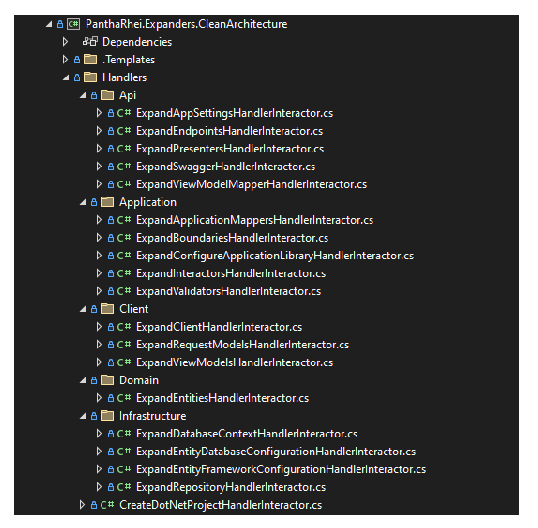
\includegraphics[width=0.6\textwidth]{figures/expander_handlers.pdf}
    \caption[handlers]{Each of the handlers handles an isolated part of the expanding process.}
    \label{fig_handlers}
\end{figure}
\subsection{Open/Closed Principle}

\evaluatePrincipleTable{\acrshort{ocp}}{table_ocp_convergence}{ 
    
\addEvalRow{\gls{soc} & \fullConvergence & The \gls{ocp} strongly converges with
    the \gls{soc} principle of \gls{ns}. \gls{ocp} states that software architectures
    should be open for extension but closed for modification. When applying \gls{ocp}
    correctly, the architecture supports new requirements built as an extension, affecting
    as few existing implementations as possible. Conversely, adhering to \gls{soc} does
    not guarantee adherence to \gls{ocp}, as \gls{soc} focuses on modularization and
    encapsulation rather than the extensibility of functionality. The same example with
    the Tasks provided in sub-section \ref{srp} is also an excellent manifestation of this
    principle.} 
    
\addEvalRow{\gls{dvt} & \noConvergence & The \gls{ocp} indirectly relates to the \gls{dvt}
principle. The convergence of both principles is weak, and no manifestations are found in
the artifacts.}
    
\addEvalRow{\gls{avt} & \fullConvergence & The \gls{ocp} strongly converges with the
    \gls{avt} principle of \gls{ns}, as both principles emphasize the importance of
    allowing changes or extensions to actions without affecting existing implementations.
    \gls{ocp} is also closely related to \gls{srp}. Besides \gls{srp}, \gls{ocp} has the
    most manifestations in the artifact, some of which are already mentioned in previous
    examples. } 
    
\addEvalRow{\gls{sos} & \noConvergence & The \gls{ocp} indirectly relates to the \gls{sos}
    principle. The convergence of both principles is weak, and no manifestations are found
    in the artifacts. } }
\subsection{Liskov Substitution Principle}

\evaluatePrincipleTable{\gls{lsp}}{table_lsp_alignment}{ 
    
\addEvalRow{\gls{soc} & \fullAlignment & \gls{lsp} states that objects of a derived class should be
able to replace objects of the base class without affecting the program negatively.
Replacing objects can only be achieved by separating them, aligning the principles
inherritly. A good example is the implementation of the
\citecode{koks_itemplateinteractor_2023} where the template engine Scriban
\parencite{github_scriban_2023} is used to generate code instantiations as a result of the
Expanding the Model \parencite{koks_scribantemplateinteractor_2023}. We could easily
replace the Scriban template engine for an other engine with only impacting the Dependency
Injection Register.}
    
\addEvalRow{\gls{dvt} & \noAlignment & The alignment between \gls{lsp} and \gls{dvt} is weak,
and no manifestations are found in the artifacts.}
    
\addEvalRow{\gls{avt} & \partialAlignment & The \gls{lsp} supports the \gls{avt} principle.
Both principles emphasize the importance of allowing the extensibility of the software
system. By adhering to \gls{lsp}, the architecture allows for class hierarchies that can
be easily extended to accommodate new (versions of) actions, which can contribute to
achieving \gls{avt}. However, adhering to \gls{lsp} alone may not guarantee full adherence
with \gls{avt}. Considder \citecode{koks_icreategateway_2023} in Code Listing
\ref{list_ICreateGatewayExamples}. The artifact contains multiple implementations of this
interface. Each implementation could be considered a different version applied to the
interface.} 
    
\addEvalRow{\gls{sos} & \noAlignment & The \gls{lsp} does not relate to the \gls{sos}
principle. The alignment of both principles is weak, and no manifestations are found in
the artifacts.} }

\subsection{Interface Segregation Principle}

\evaluatePrincipleTable{\gls{isp}}{table_isp_convergence}{ 
    
\addEvalRow{\gls{soc} & \fullConvergence & The \gls{isp} strongly converges with the
\gls{soc} principle, as both emphasize the importance of modularity and the separation of
concerns. \gls{isp} states that clients should not be forced to depend on implementation
they do not use, promoting the creation of smaller, focused interfaces. Listing
\ref{list_ispexample} shows that each \gls{crud} operation has its own interface
\parencite{koks_crudgateways_2023}.}
    
\addEvalRow{\gls{dvt} & \noConvergence & The \gls{isp} does not relate to the \gls{dvt}
principle. The convergence of both principles is weak, and no manifestations are found in
the artifacts.}
    
\addEvalRow{\gls{avt} & \npartialConvergence & The convergence between \gls{isp} and
\gls{avt} arises from the emphasis of \gls{isp} on creating targeted interfaces tailored
to specific needs. Smaller interfaces can enhance modularity and minimize unwanted side
effects when modifying Actions in the software system, positively impacting the
implementation of the \gls{avt}. For example, modifications in Actions are likely to have
a limited impact. However, adhering to \gls{isp} is not a guarantee for \gls{avt}.} 
    
\addEvalRow{\gls{sos} & \noConvergence & The \gls{isp} does not relate to the \gls{sos}
principle. The convergence of both principles is weak, and no manifestations are found in
the artifacts.} 

}
\subsubsection{The Dependency Inversion Principle} \label{subsubsec_dip} 
\textcolor{red}{
TODO: explain how dependency injection can benefit the implementation and align with
\ref{tab_convergence_dip}}

The \gls{dip} prescribes that high-level modules should not depend on low-level modules,
and that both should depend on abstractions. The principle emphasizes that the
architecture should be designed in such a way that the flow of control between the
different objects, layers and components are always from higher-level implementations
to lower-level details.

In other words, high-level implementations like business rules, should not be concerned
about low-level implementations, such as the way the data is stored or presented to the
end user. Additionally, both the high-level and low-level implementations should only
depend on abstractions or interfaces that define a contract for how they should interact
with each other \parencite[109]{robert_c_martin_clean_2018}.

This approach allows for great flexibility and a modular architecture. Modifications in
the low-level implementations will not affect the high-level implementations as long as
they still adhere to the contract defined by the abstractions and interfaces.
Similarly, changes to the high-level modules will not affect the low-level modules as long
as they still fulfill the contract. This reduces coupling and ensures the evolvability
system over time, as changes can be made to specific modules without affecting the rest of
the system.

Manifestations in the artifacts are ample. One of which is the consistent use of the
Dependency Injection pattern. In order to prevent the risks of displacing and dispersing
dependencies all over the system \parencite[214]{mannaert_normalized_2016} we are using
dependency containers. Each module is maintaining its own dependencies, which are
bootstrapped at application startup (see Listing \ref{list_dip})
\parencite{koks_generator_2023}.

\lstinputlisting[
    caption={Bootstrapping the dependencies of each component/layer of the
    generator artifact.},
    label={list_dip}]
    {Snippets/Dip.cs}

A more abstract example is the separation of required modules into separate component
libraries. This applies to both the generated and generator artifact (see Figure
\ref{fig_solutions}). The actual compliance to the \gls{dip} is how the flow of control
between the components is organized. This is accurately depicted in Figure
\ref{fig_modulair_components} \nameref{fig_modulair_components}.

\begin{figure}[H]
    \centering
    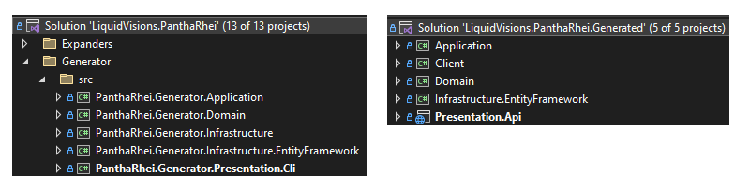
\includegraphics[width=1\textwidth]{figures/solutions.pdf}
    \caption[Separation of component libraries]{Separation of component libraries.}
    \label{fig_solutions}
\end{figure}
\subsection{The Entity Element}

\evaluateElementTable{Entity}{tab_convergence_entity}{ \addEvalRow{Data & \fullAlignment &
    Both elements represent data objects that are part of the ontology or data schema of
    the application, and typically include attributes and relationship information. While
    both can contain a full set of attributes and relationships, the Data Element of
    \gls{ns} may also be tailored to serve a specific set of information that is required
    for a single task or use case. In \gls{ca} these type of Data Elements are specified
    explicitly as ViewModels, RequestModels or ResponseModels. Code Listing
    \ref{list_entity} illustrates the similarities of between an \glspl{ca} Entity and the
    Data Element from \gls{ns} }

    \addEvalRow{Task & \noAlignment & The Entity has no alignment with the Task element of
        \gls{ns}. However, the Tasks element might operate on entities to perform business
        logic.}

    \addEvalRow{Flow & \noAlignment & The Entity and Flow elements are not aligned, as the
        Flow element represents the control between Tasks in \gls{ns}, while the Entity in
        \gls{ca} represents domain objects.}

    \addEvalRow{Connector & \noAlignment & The Entity and Connector element from \gls{ns}
        are not aligned, as the Connector element in \gls{ns} is involved in the
        communication separation of between components, while the Entity in \gls{ca}
        represents domain objects.}
    
    \addEvalRow{Trigger & \noAlignment & The Entity element and Trigger element are not convergent,
        as the Trigger element in \gls{ns} is about event-based execution of Tasks, while
        the Entity in \gls{ca} represents domain objects.}
}
\subsection{The Interactor Element}

\evaluateElementTable{Interactor}{tab_convergence_interactor}{ \addEvalRow{Data &
    \noConvergence &  There is no convergence between the Interactor element of \gls{ca} and
    the Data element of \gls{ns}, and no manifestations are found in the artifact.}

    \addEvalRow{Task & \fullConvergence &  The Interactor element of \gls{ca} has a strong
    convergence with the task element of \gls{ns}, as both encapsulate the execution
    of business rules. This is illustrated in Code Listing \ref{list_interactor_task},
    which converges with an implementation of a task, having a single execution of a business
    rule \parencite{koks_createentityvalidator_2023}. }

    \addEvalRow{Flow & \fullConvergence & The Interactor strongly converges with the Flow
        element of \gls{ns}, as both elements can orchestrate the flow of execution for a
        use case, which can involve multiple Tasks in \gls{ns}. This is clearly
        illustrated in Code Listing \ref{list_interactor_flow}, where the Interactor
        handles validation, mapping, and persistence of the Entity
        \parencite*{koks_createentityinteractor_2023}. }

    \addEvalRow{Connector & \noConvergence & There is no convergence between the Interactor
    element of \gls{ca} and the Connector element of \gls{ns}, and no manifestations are
    found in the artifact.}
    
    \addEvalRow{Trigger & \noConvergence & There is no convergence between the Interactor
    element of \gls{ca} and the Trigger element of \gls{ns}, and no manifestations are
    found in the artifact.} }
\input{chapters/evaluation/elements/requestmodel}
\input{chapters/evaluation/elements/responsemodel}
\input{chapters/evaluation/elements/viewmodel}
\subsection{The Controller Element} \label{converging_controller_element}

\evaluateElementTable{Controller}{tab_convergence_controller}{
    \addEvalRow{Data & \noAlignment & The Controllers and Data elements are not directly convergent, as
        the Controller element is focused on handling input/output from external systems, while Data
        elements represent domain objects.}

    \addEvalRow{Task & \noAlignment &  The Controllers and Task elements are not convergent. However,
        controllers might initiate Task elements when handling incoming requests.}

    \addEvalRow{Flow & \noAlignment &  The Controllers and Flow elements are not convergent, as
        the Controller element is focused on handling input/output from external systems,
        whilst the Flow element is concerned with the orchestration of Tasks.}

    \addEvalRow{Connector & \partialAlignment & The Controller and Connector element are convergent to some
        degree. Both elements are involved in communication between components. The use of
        the Controller is a bit more strict it strictly defines communication from
        external parts of the systems, involving specific Interactor.}
    
    \addEvalRow{Trigger & \partialAlignment & The Controller and the Trigger element of \gls{ns} are
        convergent to some degree as they both can initiate actions based on external
        events or requests. A Controller is primarily involved in receiving events or
        reqeusts from external sources, followed by the invocation of the appropriate
        interactor.}
}
\subsection{The Gateway Element}

\evaluateElementTable{Gateway}{tab_convergence_gateway}{ \addEvalRow{ Data & \noConvergence
    &  There is no convergence between the Gateway element of \gls{ca} and the Data element
    of \gls{ns} and no manifestations are found in the artifact.}

    \addEvalRow{Task & \noConvergence &  There is no convergence between the Gateway element
    of \gls{ca} and the task element of \gls{ns}, and no manifestations are found in the
    artifact}

    \addEvalRow{Flow & \noConvergence & There is no convergence between the Gateway element of
    \gls{ca} and the Flow element of \gls{ns}, and no manifestations are found in the
    artifact}

    \addEvalRow{Connector & \fullConvergence & The Gateway element of \gls{ca} has a strong
    convergence with the Connector element of \gls{ns}, as both are involved in
    communication between components and provide interfaces for accessing external
    resources or systems. Code Listing \ref{list_ICreateGatewayExamples} is an example of
    two different type of Gateways. The \citecode{koks_harvestrepository_2023} interacts
    with the File system of the operating system, while
    \citecode{koks_genericrepository_2023} interacts with a SQL Database. }
    
    \addEvalRow{Trigger & \noConvergence & There is no convergence between the Gateway element
    of \gls{ca} and the Trigger element of \gls{ns}, and no manifestations are found in the
    artifact} }
\subsection{The Presenter Element}

\evaluateElementTable{Presenter}{tab_convergence_presenter}{ \addEvalRow{Data &
    \noAlignment &  There is no alignment between the Presenter and the Task Element of
    \gls{ns}.}

    \addEvalRow{Task & \partialAlignment &  The Presenter is responsible for in preparing the
    Response and ViewModel on behalf of the Controller and can be considdered a Task Element with a
    very specialized job. Code Listing \ref{list_createentitypresenter} illustrated the
    inner workings of a Presenter \parencite{koks_createentitypresenter_2023}}

    \addEvalRow{Flow & \partialAlignment & Presenters can handle multiple Tasks when this
    is required. in this case there is also some alignment between the Presenter Element
    of \gls{ca} with the Flow Element of \gls{ns}.}

    \addEvalRow{Connector & \noAlignment & There is no alignment between the Presenter
    and the Connector Element of \gls{ns}.}
    
    \addEvalRow{Trigger & \noAlignment & There is no alignment between the Presenter
    and the Trigger Element of \gls{ns}.}
}
\subsection{The Boundary Element}

\evaluateElementTable{Boundary}{tab_convergence_boundary}{ \addEvalRow{Data & \noConvergence
    &  There is no convergence between the Boundary element of \gls{ca} and the Data
    element of \gls{ns}, and no manifestations are found in the artifact.}

    \addEvalRow{ Task & \noConvergence &  There is no convergence between the Boundary element
    of \gls{ca} and the task element of \gls{ns}, and no manifestations are found in the
    artifact.}

    \addEvalRow{ Flow & \noConvergence & There is no convergence between the Boundary
    element of \gls{ca} and the Flow element of \gls{ns}, and no manifestations are found
    in the artifact.}

    \addEvalRow{Connector & \fullConvergence & The Boundary element of \gls{ca} has a
    strong convergence with the Connector element of \gls{ns}, as both are involved in
    communication between components and help ensure loose coupling between these
    components. However, the Boundary element's scope seems narrower, as this element
    usually separates architectural boundaries within the application or component. In the
    Code Listing Example \ref{list_CreateEntityBoundary}, we can notice that the primary
    purpose of the Boundary is to separate the inner parts of the Application layer from
    the Presentation layer, which converges with the goal of the Connector Element of
    \gls{ns}}.
    
    \addEvalRow{ Trigger & \noConvergence & There is no convergence between the Boundary
    element of \gls{ca} and the task element of \gls{ns}, and no manifestations are found
    in the artifact.} }


